\documentclass{officialexam} 
\usepackage{pgf,tikz}
\usetikzlibrary{arrows}
\usepackage{wrapfig}
\usepackage{graphicx}
\usepackage{float}
\usepackage[table]{xcolor}
\usepackage{pgfplots}
\usepackage{esvect}
\def\tablename{តារាង}
\renewcommand{\thefigure}{\khmer{figure}}
\def\figurename{រូបទី}
\definecolor{xfqqff}{rgb}{0.5,0,1}
\definecolor{qqqqff}{rgb}{0,0,1}
\definecolor{ffqqqq}{rgb}{1,0,0}
\definecolor{qqqqff}{rgb}{0,0,1}
\begin{document}
	{\maketitle}
	\borderline{ប្រធាន ០១}
	\begin{enumerate}[I]
		\item គណនាមាឌធុងដែលផ្ទុកឧស្ម័នអុកសុីសែន $9.6g$ នៅសម្ពាធ $10^5Pa$ និងសីតុណ្ហភាព $300K$។ គេឲ្យ៖ $R=8.31J/mol\cdot K$ និងម៉ាសម៉ូលនៃឧស្ម័នអុកសុីសែន$32g/mol$ ។
		\item ចលនាផង់ផ្ទុកបន្ទុកអគ្គិសនីស្ថិតក្នុងដែនម៉ាញេទិចឯកសណ្ឋាន $\vec{B}$ ក្នុងករណី $\vec{v}$ ស្រប $\vec{B}$ $\vec{v}$ កែង $\vec{B}$ $\vec{v}$ និង$\vec{B}$ បង្កើតបានមុំ $\alpha\left(0<\alpha<90^\circ\right)$។ តើករណីនីមួយៗចលនារបស់ផង់មានគន្លងដូចម្តេច?
		\item កំណត់កម្តៅភាយចេញពីប្រព័ន្ធ បើខ្យល់ត្រូវបានបង្រួមតាមលំនាំអុីសូទែមពីមាឌ $50L$ នៅសម្ពាធធម្មតា $1atm$ ចុះមកដល់មាឌ $10L$។ គេឲ្យ៖ $\ln1.5=0.40,\ln1=0, \ln2=0.7, \ln5=1.6$ ។
		\item ម៉ាសុីនកាកណូមួយបានបំពេញកម្មន្ត $W=1500J$ ក្នុងសុិកនីមួយៗ នៃដំណើរការ $t=0.25s$ នៅចន្លោះសីតុណ្ហភាព $T_h=850K$ និង $T_c=340K$ ។
		\begin{enumerate}[k]
			\item គណនាទិន្នផលនៃម៉ាសុីននេះ។
			\item គណនាតម្លៃមធ្យមនៃអនុភាពម៉ាសុីន។
			\item គណនាបរិមាណកំដៅដែលផ្ដល់ដោយធុងដែលមានសីតុណ្ហភាពខ្ពស់។
			\item គណនាបរិមាណកម្តៅដែលទទួលបានដោយធុងដែលមានសីតុណ្ហភាពទាប។
		\end{enumerate}
		\item បម្លាស់ទីនៃរលកមួយមានសមីការ $y=0.30\sin\left(0.20x-0.20t\right)(m)$។ ចូរគណនា៖\\
		អំព្លីទុតនៃរលក ចំនួនរលក ជំហានរលក ខួបនៃរលក និងល្បឿនដំណាលនៃរលក។
		\item សូលេណូអុីតមួយមានប្រវែង $50cm$ រុំដោយខ្សែចម្លងឆ្មារដែលមានអង្កត់ផ្ចិត $0.8mm$ ស្រោបដោយអុីសូឡង់ដែលមានកម្រាស់ $0.1mm$ ជាស្ពៀជាប់ៗគ្នា។ គេឲ្យ៖ ជំរាបម៉ាញេទិច $\mu_0=4\pi\times10^{-7}T\cdot m/A$ 
		\begin{enumerate}[k]
			\item គណនាចំនួនស្ពៀនៃសូលេណូអុីត
			\item គណនាដែនម៉ាញេទិចដែលកើតមានត្រង់ផ្ចិតនៃសូលេណូអុីត បើវាឆ្លងកាត់ដោយចរន្ត $10A$ 
		\end{enumerate}
		\item ខ្សែចម្លងត្រង់មួយឆ្លងកាត់ដោយចរន្ត $2.5A$។ ចូរកំណត់វុិចទ័រអាំងឌុចស្យុងម៉ាញេទិចត្រង់ចំណុចមួយដែលស្ថិតនៅចម្ងាយ $10cm$ ពីខ្សែ និងគូសរូបបញ្ជាក់ផង។
		\item អេឡិចត្រុងមួយមានល្បឿន $v=10^{6}m/s$ ធ្វើចលនាចូរក្នុងដែនម៉ាញេទិចឯកសណ្ឋានដែលមានអាំងឌុចស្យុង $B=8\times10^{-4}T$។ តាមទិសកែងនឹងខ្សែដែនម៉ាញេទិច។
		\begin{enumerate}[k]
			\item គណនាកាំគន្លងរបស់អេឡិចត្រុងពេលផ្លាស់ទីចូរដែនម៉ាញេទិចឯកសណ្ឋាន។
			\item គណនារយៈពេល ដែលអេឡិចត្រុងផ្លាស់ទីបានកន្លះជុំ។
			\item គណនាបម្រែបម្រួលថាមពលសុីនេទិច ពេលដែលល្បឿនរបស់វាថេរ។
		\end{enumerate}
	\end{enumerate}
\borderline{ចម្លើយ}\\
{\color{white}.}\dotfill\\
{\color{white}.}\dotfill\\
{\color{white}.}\dotfill
\\
{\color{white}.}\dotfill\\
{\color{white}.}\dotfill\\
{\color{white}.}\dotfill
\\
{\color{white}.}\dotfill\\
{\color{white}.}\dotfill\\
{\color{white}.}\dotfill
\\
{\color{white}.}\dotfill\\
{\color{white}.}\dotfill\\
{\color{white}.}\dotfill
\\
{\color{white}.}\dotfill\\
{\color{white}.}\dotfill\\
{\color{white}.}\dotfill
\\
{\color{white}.}\dotfill\\
{\color{white}.}\dotfill\\
{\color{white}.}\dotfill
\\
{\color{white}.}\dotfill\\
{\color{white}.}\dotfill\\
{\color{white}.}\dotfill
\\
{\color{white}.}\dotfill\\
{\color{white}.}\dotfill\\
\begin{center}
	\sffamily\color{blue}
	សូមសំណាងល្អ!
\end{center}\newpage
{\maketitle}
\borderline{ប្រធាន ០២}
\begin{enumerate}[I]
	\item គណនាកម្លាំងម៉ាញេទិចដែលមានអំពើលើយន្តហោះមួយផ្ទុកបន្ទុកអគ្គិសនី $150C$ កំពុងហោះហើរដោយល្បឿន $350m/s$ កែងនឹងទិសដៅដែនម៉ាញេទិចផែនដីដែលមានតម្លៃ $2.0\times10^{-5}T$ ។
	\item បម្លាស់ទីនៃចលនាមួយមានសមីការ $y=0.20\sin60\pi\left(10t-x\right)$ ដែល $x, y$ គិតជា $m$ និង $t$ គិតជា $s$\\
	ចូរកំណត់ អំព្លីទុត ខួប ប្រេកង់ ល្បឿនដំណាល និងជំហានរលកនៃបម្លាស់ទីនេះ។
	\item សុីឡាំងនៃម៉ាសុីនមួយមានមុខកាត់ $A=6dm^2$ នៅភាពដើមឧស្ម័នមានមាឌ $V_1=0.9dm^3$។ \\ក្រោមសម្ពាធថេរ $P=20\times10^5Pa$ ឧស្ម័នបំពេញកម្មន្តទៅលើពីស្តុងឲ្យផ្លាស់ទីបានចម្ងាយ $d=0.1dm$។
	\begin{enumerate}[k]
		\item គណនាបម្រែបម្រួលមាឌក្នុងពេលដែលឧស្ម័នបំពេញកម្មន្ត។ រូចទាញរកមាឌស្រេច។
		\item គណនាកម្នន្តដែលបានបំពេញដោយឧស្ម័ន។
		\item គណនាបម្រែបម្រួលថាមពលក្នុង។ បើឧស្ម័នដែលស្ថិតក្នុងសុីឡាំងនេះមានចំនួនម៉ូល $n=2mol$ ។
	\end{enumerate} 
	\item គណនាបម្រែបម្រួលថាមពលក្នុងរបស់ប្រព័ន្ធឌែម៉ូឌីណាមិចក្នុងលក្ខខណ្ឌដូចខាងក្រោម៖
	\begin{enumerate}[k]
		\item ក្នុងពេលតែមួយប្រព័ន្ធស្រូបកម្តៅ $500cal$ និងធ្វើកម្មន្ត $400J$។
		\item ក្នុងពេលតែមួយប្រព័ន្ធស្រូបកម្តៅ $300cal$ និងទទួលកម្មន្តពីធុងក្រៅ $420J$
		\item ប្រព័ន្តបញ្ចេញកម្តៅ $1200cal$ ដោយរក្សាមាឌថេរ។ គេឲ្យ៖ $1cal=4.19J$
	\end{enumerate}
	\item គេឲ្យរលកពីរដាលដោយទិសដៅដូចគ្នា ប្រេកង់ដូចគ្នា មានអំព្លីទុត $a_1=a_2=4cm$ ផាសដើម $\phi_1=3\pi$ និង $\phi_2=\frac{\pi}{2}$។
	\begin{enumerate}[k]
		\item ចូរសរសេរសមីការរលកសុីនុយសូអុីតនីមួយៗ។
		\item ចូរសរសេរសមីការរលកតម្រួតនៃរលកទាំងពីរ។
		\item កំណត់អំព្លីទុតតម្រួត និងផាសដើមតម្រួតនៃរលក។
	\end{enumerate}
	\item ខ្សែចម្លងពីរដាក់ស្របគ្នាប្រវែងស្មើគ្នាឆ្លងកាត់ដោយចរន្តដែលមានទិសដៅដូចគ្នា និងមានអាំងតង់សុីតេស្មើគ្នា $I=10A$ ហើយប្រវែងខ្សែចម្លងនីមួយៗគឺ $l_1=l_2=l=2m$។ ខ្សែចម្លងទាំងពីររងនូវកម្លាំង $F=4\times10^{-4}N$។
	\begin{enumerate}[k]
		\item ធ្វើគំនូសតាងវុិចទ័រ ដែនម៉ាញេទិច $\vec{B}$ និងកម្លាំងអេឡិចត្រូម៉ាញេតិច $\vec{F}$។
		\item គណនាចម្ងាយរវាងខ្សែចម្លងទាំងពីរ។
	\end{enumerate}
	\item សូលេណូអុីតមួយមានប្រវែង $50cm$ មានអង្កត់ផ្ចិត $2cm$ និងចំនួនស្ពៀ $1000$ រុំដោយខ្សែចម្លងដែលមានមុខកាត់ $1mm^2$ មានរេសុីស្ទីវីតេ $\rho=1.6\mu\Omega cm$
	\begin{enumerate}[k]
		\item គណនារេសុីស្តង់នៃសូលេណូអុីត
		\item គណនាអាំងឌុចស្យុងម៉ាញេទិចក្នុងសូលេណូអុីត បើចរន្ត $10A$ ឆ្លងកាត់សូលេណូអុីត។
		\item គណនាផលសងប៉ូតង់ស្យែលនៃសូលេណូអុីតនេះ។
	\end{enumerate}
\end{enumerate}
\borderline{ចម្លើយ}\\
{\color{white}.}\dotfill\\
{\color{white}.}\dotfill\\
{\color{white}.}\dotfill
\\
{\color{white}.}\dotfill\\
{\color{white}.}\dotfill\\
{\color{white}.}\dotfill
\\
{\color{white}.}\dotfill\\
{\color{white}.}\dotfill\\
{\color{white}.}\dotfill
\\
{\color{white}.}\dotfill\\
{\color{white}.}\dotfill\\
{\color{white}.}\dotfill
\\
{\color{white}.}\dotfill\\
{\color{white}.}\dotfill\\
{\color{white}.}\dotfill
\\
{\color{white}.}\dotfill\\
{\color{white}.}\dotfill\\
{\color{white}.}\dotfill
\\
{\color{white}.}\dotfill\\
{\color{white}.}\dotfill\\
{\color{white}.}\dotfill
\\
{\color{white}.}\dotfill\\
{\color{white}.}\dotfill\\
\begin{center}
	\sffamily\color{blue}
	សូមសំណាងល្អ!
\end{center}\newpage
{\maketitle}
\borderline{ប្រធាន ០៣}
\begin{enumerate}[I]
	\item តើម៉ូទ័រចំហេះមានប៉ុន្មានប្រភេទ? មានអ្វីខ្លះ? ចូររៀបរាប់ប្រភេទនីមួយៗ។
	\item គណនាមាឌឧស្ម័នអុកសុីសែន $3.2g$ ដែលផ្ទុកក្នុងធុងនៅសម្ពាធ $76cmHg$ និងសីតុណ្ហភាព $27^\circ$។ \\គេឲ្យ ថេរសកល $R=8.31J/mol\cdot K$ និងម៉ាសម៉ូលនៃអុកសុីសែន $32g/mol$
	\item គេឲ្យដ្យាក្រាមដូចរូប
	\begin{multicols}{2}
			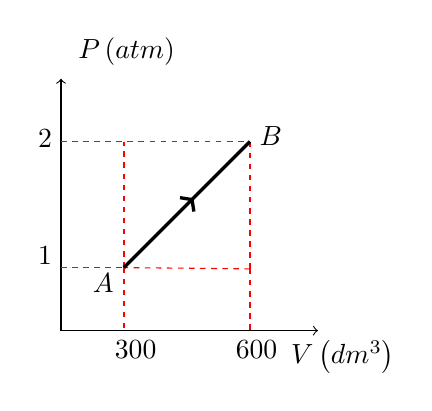
\begin{tikzpicture}[x=1.0cm,y=1.0cm, scale=.80]
			\draw [->] (0,-1) -- (0,3);
			\draw [->] (0,-1) -- (4.08,-1);
			\draw [dash pattern=on 2pt off 2pt, color=ffqqqq] (1,0)-- (1,2);
			\draw [dash pattern=on 2pt off 2pt, color=ffqqqq] (1,0)-- (1,-1);
			\draw [dash pattern=on 2pt off 2pt, color=ffqqqq] (0,0)-- (1,0);
			\draw [dash pattern=on 2pt off 2pt,color=ffqqqq] (0,2)-- (3,2);
			\draw [dash pattern=on 2pt off 2pt, color=ffqqqq] (3,2)-- (3,-0.02);
			\draw [dash pattern=on 2pt off 2pt, color=ffqqqq] (3,-0.02)-- (1,0);
			\draw [dash pattern=on 2pt off 2pt, color=ffqqqq] (3,-0.02)-- (3,-1);
			\draw [line width=1.2pt] (1,0)-- (3,2);
			\draw [line width=1.2pt] (2.08,1.08) -- (2.11,0.89);
			\draw [line width=1.2pt] (2.08,1.08) -- (1.89,1.11);
			\draw (0.12,3.8) node[anchor=north west] {$ P\left(atm\right) $};
			\draw (3.50,-1) node[anchor=north west] {$ V\left(dm^3\right) $};
			\draw (3.0,2.40) node[anchor=north west] {$ B $};
			\draw (0.35,0.06) node[anchor=north west] {$ A $};
			\draw (0.70,-1) node[anchor=north west] {$300$};
			\draw (2.62,-1) node[anchor=north west] {$600$};
			\draw (-0.52,2.34) node[anchor=north west] {$2$};
			\draw (-0.52,0.48) node[anchor=north west] {$1$};
			\end{tikzpicture}
		\begin{enumerate}[k]
			\item គណនាកម្មន្តដែលបានបំពេញដោយឧស្ម័ននោះ។
			\item គណនាបម្រែបម្រួលថាមពលក្នុងរបស់ប្រព័ន្ធ។
			\item គណនាកម្តៅដែលស្រូបដោយប្រព័ន្ធក្នុងរយៈពេលបម្រែបម្រួលមាឌនេះ។
		\end{enumerate}
	\end{multicols}
	\item រករលកតម្រួតនៃលំយោលខាងក្រោម៖
	\begin{enumerate}[k]
		\item $y_1=6\sin\left(7\pi t + \frac{\pi}{2}\right)\left(cm\right)$ និង $y_2=6\sin\left(7\pi t + \frac{\pi}{6}\right)​\left(cm\right)$
		\item  $y_1=8\sin\left(10t + \frac{\pi}{2}\right)\left(cm\right)~;~y_2=8\sin\left(10t\right)\left(cm\right)$ និង $y_3=8\sin\left(10t - \frac{\pi}{2}\right)\left(cm\right)$
	\end{enumerate}
	\item រាល់វិនាទីម៉ូទ័ររថយន្តមួយទទួលកម្តៅ $172kJ$ ពីប្រតិកម្មចំហេះល្បាយឧស្ម័ន និងបញ្ចេញមកបរិយាកាស $135kJ$។
	\begin{enumerate}[m]
		\item \begin{enumerate}[k]
			\item រៀបរាប់វគ្គទាំងបួននៃសិុច។
			\item គណនាកម្មន្តមេកានិច ក្នុងរយៈពេល $10mn$។
			\item គណនាទិន្នផលកម្តៅនៃម៉ូទ័រ។ 
		\end{enumerate}
		\item ទិន្នផលគ្រឿងបញ្ជួនគឺ $92\%$។
		\begin{enumerate}[k]
			\item គណនាកម្មន្តបានការដែលភ្លៅម៉ូទ័រទទួល។
			\item គណនាទិន្នផលបានការនៃម៉ាសុីន។
		\end{enumerate}
	\end{enumerate}\newpage
	\item គេចង់បង្កើតសូលេណូអុីតមួយដែលមានរេសុីស្តង់ $5.0\Omega$ និងអាចបង្កើតដែន $4.0\times10^{-2}T$ ពេលមានចរន្ត $4.0A$ ឆ្លងកាត់។ សូលេណូអុីតនេះត្រូវបានរុំពីខ្សែចម្លងទង់ដែងដែលមានអង្កត់ផ្ចិត $0.50mm$។ ប្រសិនបើសូលេណូអុីតមានកាំ $1.0cm$។ គណនា៖
	\begin{enumerate}[k]
		\item ចំនួនស្ពៀខ្សែចម្លងដែលរុំជាសូលេណូអុីត។
		\item ប្រវែងសូលេណូអុីត។
		\item ផលសងប៉ូតង់ស្យែលនៃគោលទាំងពីររបស់សូលេណូអុីត។
	\end{enumerate}
\end{enumerate}
\borderline{ចម្លើយ}\\
{\color{white}.}\dotfill\\
{\color{white}.}\dotfill\\
{\color{white}.}\dotfill
\\
{\color{white}.}\dotfill\\
{\color{white}.}\dotfill\\
{\color{white}.}\dotfill
\\
{\color{white}.}\dotfill\\
{\color{white}.}\dotfill\\
{\color{white}.}\dotfill
\\
{\color{white}.}\dotfill\\
{\color{white}.}\dotfill\\
{\color{white}.}\dotfill
\\
{\color{white}.}\dotfill\\
{\color{white}.}\dotfill\\
{\color{white}.}\dotfill
\\
{\color{white}.}\dotfill\\
{\color{white}.}\dotfill\\
{\color{white}.}\dotfill
\\
{\color{white}.}\dotfill\\
{\color{white}.}\dotfill\\
{\color{white}.}\dotfill
\\
{\color{white}.}\dotfill\\
{\color{white}.}\dotfill\\
\begin{center}
	\sffamily\color{blue}
	សូមសំណាងល្អ!
\end{center}\newpage
\maketitle
\borderline{ប្រធាន ០៤}
\begin{enumerate}[m]
	\item ឧស្ម័នមួយម៉ូលទទួលបម្លែងទែម៉ូឌីណាមិចតាមលំនាំអុីសូទែម ដូចរូប។
	\begin{multicols}{2}
		\begin{tikzpicture}[x=1.0cm,y=1.0cm, scale=.70]
			\draw [->,color=qqqqff] (0,-1) -- (0,4);
			\draw [->,color=qqqqff] (0,-1) -- (5,-1);
			\draw [line width=1.2pt,color=qqqqff] (2,0)-- (2,3);
			\draw [line width=1.2pt,color=qqqqff] (2,1.62) -- (2.15,1.5);
			\draw [line width=1.2pt,color=qqqqff] (2,1.62) -- (1.85,1.5);
			\draw [dash pattern=on 2pt off 2pt] (2,0)-- (2,-1);
			\draw [dash pattern=on 2pt off 2pt,color=ffqqqq] (0,0)-- (2,0);
			\draw [dash pattern=on 2pt off 2pt,color=ffqqqq] (0,3)-- (2,3);
			\draw (-0.72,3.46) node[anchor=north west] {$ 2 $};
			\draw (-0.62,0.44) node[anchor=north west] {$ 1 $};
			\draw (1.52,-1.1) node[anchor=north west] {$ 300 $};
			\draw (0.16,4.36) node[anchor=north west] {$ P\left(atm\right) $};
			\draw (4.08,-1) node[anchor=north west] {$ T\left(K\right) $};
		\end{tikzpicture}
		\begin{enumerate}[k]
			\item គណនាកម្មន្តនៃឧស្ម័ន។
			\item តើប្រព័ន្ធស្រូបកម្តៅ ឬប្រព័ន្ធបំភាយកម្តៅ?\\
			គេឲ្យ៖ $\ln1=0;\ln1.5=0.40;\ln2=0.70;\ln5=1.6$
		\end{enumerate}
	\end{multicols}
\end{enumerate}
\borderline{ចម្លើយ}\\
{\color{white}.}\dotfill\\
{\color{white}.}\dotfill\\
{\color{white}.}\dotfill
\\
{\color{white}.}\dotfill\\
{\color{white}.}\dotfill\\
{\color{white}.}\dotfill
\\
{\color{white}.}\dotfill\\
{\color{white}.}\dotfill\\
{\color{white}.}\dotfill
\\
{\color{white}.}\dotfill\\
{\color{white}.}\dotfill\\
{\color{white}.}\dotfill
\\
{\color{white}.}\dotfill\\
{\color{white}.}\dotfill\\
{\color{white}.}\dotfill
\\
{\color{white}.}\dotfill\\
{\color{white}.}\dotfill\\
{\color{white}.}\dotfill
\\
{\color{white}.}\dotfill\\
{\color{white}.}\dotfill\\
{\color{white}.}\dotfill
\\
{\color{white}.}\dotfill\\
{\color{white}.}\dotfill\\
\begin{center}
	\sffamily\color{blue}
	សូមសំណាងល្អ!
\end{center}\newpage
\end{document}